	% ========================================
%	Header einbinden
% ========================================

\documentclass[bibtotoc,titlepage]{scrartcl}

% Deutsche Spracheinstellungen
\usepackage[ngerman,german]{babel, varioref}
\usepackage[T1]{fontenc}
\usepackage[utf8]{inputenc}

%\usepackage{marvosym}

\usepackage{amsfonts}
\usepackage{amssymb}
\usepackage{amsmath}
\usepackage{amscd}
\usepackage{amstext}

\usepackage{longtable}

%\usepackage{bibgerm}

\usepackage{footnpag}

\usepackage{ifthen}                 %%% package for conditionals in TeX
\usepackage[amssymb]{SIunits}
%Für textumflossene Bilder und Tablellen
%\usepackage{floatflt} - veraltet

%Für Testzwecke aktivieren, zeigt labels und refs im Text an.
%\usepackage{showkeys}

% Abstand zwischen zwei Absätzen nach DIN (1,5 Zeilen)
% \setlength{\parskip}{1.5ex plus0.5ex minus0.5ex}

% Einrückung am Anfang eines neuen Absatzes nach DIN (keine)
%\setlength{\parindent}{0pt}

% Ränder definieren
% \setlength{\oddsidemargin}{0.3cm}
% \setlength{\textwidth}{15.6cm}

% bessere Bildunterschriften
%\usepackage[center]{caption2}


% Problemlösungen beim Umgang mit Gleitumgebungen
\usepackage{float}

% Nummeriert bis zur Strukturstufe 3 (also <section>, <subsection> und <subsubsection>)
%\setcounter{secnumdepth}{3}

% Führt das Inhaltsverzeichnis bis zur Strukturstufe 3
%\setcounter{tocdepth}{3}
\usepackage[version=3]{mhchem}
	\mhchemoptions{minus-sidebearing-left=0.06em, minus-sidebearing-right=0.11em}
\usepackage{exscale}

\newenvironment{dsm} {\begin{displaymath}} {\end{displaymath}}
\newenvironment{vars} {\begin{center}\scriptsize} {\normalsize \end{center}}


\newcommand {\en} {\varepsilon_0}               % Epsilon-Null aus der Elektrodynamik
\newcommand {\lap} {\; \mathbf{\Delta}}         % Laplace-Operator
\newcommand {\R} { \mathbb{R} }                 % Menge der reellen Zahlen
\newcommand {\e} { \ \mathbf{e} }               % Eulersche Zahl
\renewcommand {\i} { \mathbf{i} }               % komplexe Zahl i
\newcommand {\N} { \mathbb{N} }                 % Menge der nat. Zahlen
\newcommand {\C} { \mathbb{C} }                 % Menge der kompl. Zahlen
\newcommand {\Z} { \mathbb{Z} }                 % Menge der kompl. Zahlen
\newcommand {\limi}[1]{\lim_{#1 \rightarrow \infty}} % Limes unendlich
\newcommand {\sumi}[1]{\sum_{#1=0}^\infty}
\newcommand {\rot} {\; \mathrm{rot} \,}         % Rotation
\newcommand {\grad} {\; \mathrm{grad} \,}       % Gradient
\newcommand {\dive} {\; \mathrm{div} \,}        % Divergenz
\newcommand {\dx} {\; \mathrm{d} }              % Differential d
\newcommand {\cotanh} {\; \mathrm{cotanh} \,}   %Cotangenshyperbolicus
\newcommand {\asinh} {\; \mathrm{areasinh} \,}  %Area-Sinus-Hyp.
\newcommand {\acosh} {\; \mathrm{areacosh} \,}  %Area-Cosinus-H.
\newcommand {\atanh} {\; \mathrm{areatanh} \,}  %Area Tangens-H.
\newcommand {\acoth} {\; \mathrm{areacoth} \,}  % Area-cotangens
\newcommand {\Sp} {\; \mathrm{Sp} \,}
\newcommand {\mbe} {\stackrel{\text{!}}{=}}     %Must Be Equal
\newcommand{\qed} { \hfill $\square$\\}
\renewcommand{\i} {\imath}
\def\captionsngerman{\def\figurename{\textbf{Abb.}}}

%%%%%%%%%%%%%%%%%%%%%%%%%%%%%%%%%%%%%%%%%%%%%%%%%%%%%%%%%%%%%%%%%%%%%%%%%%%%
% SWITCH FOR PDFLATEX or LATEX
%%%%%%%%%%%%%%%%%%%%%%%%%%%%%%%%%%%%%%%%%%%%%%%%%%%%%%%%%%%%%%%%%%%%%%%%%%%%
%%%
\ifx\pdfoutput\undefined %%%%%%%%%%%%%%%%%%%%%%%%%%%%%%%%%%%%%%%%% LATEX %%%
%%%
\usepackage[dvips]{graphicx}       %%% graphics for dvips
\DeclareGraphicsExtensions{.eps,.ps}   %%% standard extension for included graphics
\usepackage[ps2pdf]{thumbpdf}      %%% thumbnails for ps2pdf
\usepackage[ps2pdf,                %%% hyper-references for ps2pdf
bookmarks=true,%                   %%% generate bookmarks ...
bookmarksnumbered=true,%           %%% ... with numbers
hypertexnames=false,%              %%% needed for correct links to figures !!!
breaklinks=true,%                  %%% breaks lines, but links are very small
linkbordercolor={0 0 1},%          %%% blue frames around links
pdfborder={0 0 112.0}]{hyperref}%  %%% border-width of frames
%                                      will be multiplied with 0.009 by ps2pdf
%
\hypersetup{ pdfauthor   = {Hannes Franke; Julius Tilly},
pdftitle    = {V301 Innenwiderstand und Leistungsanpassung}, pdfsubject  = {Protokoll FP}, pdfkeywords = {V301, Innenwiderstand, Leistungsanpassung},
pdfcreator  = {LaTeX with hyperref package}, pdfproducer = {dvips
+ ps2pdf} }
%%%
\else %%%%%%%%%%%%%%%%%%%%%%%%%%%%%%%%%%%%%%%%%%%%%%%%%%%%%%%%%% PDFLATEX %%%
%%%
\usepackage[pdftex]{graphicx}      %%% graphics for pdfLaTeX
\DeclareGraphicsExtensions{.pdf}   %%% standard extension for included graphics
\usepackage[pdftex]{thumbpdf}      %%% thumbnails for pdflatex
\usepackage[pdftex,                %%% hyper-references for pdflatex
bookmarks=true,%                   %%% generate bookmarks ...
bookmarksnumbered=true,%           %%% ... with numbers
hypertexnames=false,%              %%% needed for correct links to figures !!!
breaklinks=true,%                  %%% break links if exceeding a single line
linkbordercolor={0 0 1},
linktocpage]{hyperref} %%% blue frames around links
%                                  %%% pdfborder={0 0 1} is the default
\hypersetup{
pdftitle    = {V301 Innenwiderstand und Leistungsanpassung}, 
pdfsubject  = {Protokoll AP}, 
pdfkeywords = {V301, Innenwiderstand, Leistungsanpassung},
pdfsubject  = {Protokoll AP},
pdfkeywords = {V301, Innenwiderstand, Leistungsanpassung}}
%                                  %%% pdfcreator, pdfproducer,
%                                      and CreationDate are automatically set
%                                      by pdflatex !!!
\pdfadjustspacing=1                %%% force LaTeX-like character spacing
\usepackage{epstopdf}
%
\fi %%%%%%%%%%%%%%%%%%%%%%%%%%%%%%%%%%%%%%%%%%%%%%%%%%% END OF CONDITION %%%
%%%%%%%%%%%%%%%%%%%%%%%%%%%%%%%%%%%%%%%%%%%%%%%%%%%%%%%%%%%%%%%%%%%%%%%%%%%%
% seitliche Tabellen und Abbildungen
%\usepackage{rotating}
\usepackage{ae}
\usepackage{
  array,
  booktabs,
  dcolumn
}
\makeatletter 
  \renewenvironment{figure}[1][] {% 
    \ifthenelse{\equal{#1}{}}{% 
      \@float{figure} 
    }{% 
      \@float{figure}[#1]% 
    }% 
    \centering 
  }{% 
    \end@float 
  } 
  \makeatother 


  \makeatletter 
  \renewenvironment{table}[1][] {% 
    \ifthenelse{\equal{#1}{}}{% 
      \@float{table} 
    }{% 
      \@float{table}[#1]% 
    }% 
    \centering 
  }{% 
    \end@float 
  } 
  \makeatother 
%\usepackage{listings}
%\lstloadlanguages{[Visual]Basic}
%\allowdisplaybreaks[1]
%\usepackage{hycap}
%\usepackage{fancyunits}

\usepackage{float}
\usepackage{caption}
\usepackage{wrapfig}

\newfloat{formel}{htbp}{for}
\floatname{formel}{Formel}

% ========================================
%	Angaben für das Titelblatt
% ========================================

\title{Das Kugelfall Viskosimeter nach Höppler\\				% Titel des Versuchs 
\large TU Dortmund, Fakultät Physik\\ 
\normalsize Anfänger-Praktikum}

\author{Jan Adam\\			% Name Praktikumspartner A
{\small \href{jan.adam@tu-dortmund.de}{jan.adam@tu-dortmund.de}}	% Erzeugt interaktiven einen Link
\and						% um einen weiteren Author hinzuzfügen
Dimitrios Skodras\\			% Name Praktikumspartner B
{\small \href{dimitrios.skodras@tu-dortmund.de}{dimitrios.skodras@tu-dortmund.de}}		% Erzeugt einen interaktiven Link
}
\date{04.12.12}					% Das Datum der Versuchsdurchführung

% ========================================
%	Das Dokument beginnt
% ========================================

\begin{document}

% ========================================
%	Titelblatt erzeugen
% ========================================

\maketitle					% Jetzt wird die Titelseite erzeugt
\thispagestyle{empty} 				% Weder Kopfzeile noch Fußzeile

% ========================================
%	Der Vorspann
% ========================================

%\newpage					% Wenn Verzeichnisse auf einer neuen Seite beginnen sollen
%\pagestyle{empty}				% Weder Kopf- noch Fußzeile für Verzeichnisse

\tableofcontents

%\newpage					% eine neue Seite
%\thispagestyle{empty}				% Weder Kopf- noch Fußzeile für Verzeichnisse
%\listoffigures					% Abbildungsverzeichnis

%\newpage					% eine neue Seite
%\thispagestyle{empty}				% Weder Kopf- noch Fußzeile für Verzeichnisse
%\listoftables					% Tabellenverzeichnis
\newpage					% eine neue Seite


% ========================================
%	Kapitel
% ========================================

%	\section{Einleitung}				% Bei Bedarf

	\section{Theorie}
Auf bewegte Körper in Flüssigkeiten oder Gasen wirkt, ähnlich wie auf rollende oder gleitende Körper, eine Reibungskraft
\begin{align}
\vec F_R=6 \pi \eta v r,
\label{stokes}
\end{align}
 die der Bewegung entgegen wirkt. Wichtig ist hier die Viskosität $\eta $, eine Stoffeigenschaft, die das Fließverhalten von Flüssigkeiten und Gasen beschreibt und proportional auf die Reibungskraft einwirkt. Sie ist zudem die einzige stoffspezifische Größe, die Einfluss auf die Reibungskraft hat. Die restlichen Größen hängen lediglich von der Körpergeometrie ab, so dass nach Bestimmung der Viskosität, die Reibungskraft für beliebige Körper im entsprechenden Medium berechnet werden kann.
 Zu beachten ist, dass die Stokes'sche Reibung \eqref{stokes} nur für laminare Flüssigkeiten gilt. Laminare Flüssigkeiten bilden keine Verwirbelungen, sondern umfließen den Körper homogen. Eine Flüssigkeit wird als laminar bezeichnet, wenn ihre Reynoldszahl
 \begin{align}
 Re= \frac{\rho v d}{\eta} = \frac{v d}{\nu}
 \end{align}
unter dem kritischen Wert von 2000 bleibt. Ab diesem Wert werden Flüssigkeiten nicht mehr als laminar bezeichnet, jedoch können sich Verwirbelungen schon viel früher bilden, so dass  $Re \ll 2000$ sein sollte. 
	\section{Aufbau}
\begin{wrapfigure}{r}{5cm}
	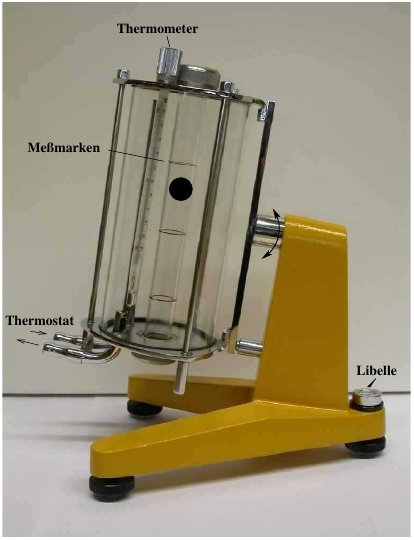
\includegraphics[width=0.35\textwidth]{pics/aufbau.jpg}
	\caption{Viskosimeter}
	\label{aufbau}
\end{wrapfigure}

Beim Kugelfall-Viskosimeters nach Höppler handelt es sich um zwei ineinander eingelassene Hohlzylinder aus Glas, welche mit Flüssigkeiten befüllt und hermetisch abgeschlossen werden können. Auf Abbildung \ref{aufbau} \footnote{Viskosimeter nach Höppler - Das Bild ist aus der Versuchsanleitung entnommen} ist das Viskosimeter zu erkennen.\\
Der innere Zylinder weißt Markierunge auf, durch die eine Strecke von 10cm abgesteckt werden. Er wird während des Versuchs mit der Flüssigkeit befüllt, deren Viskosität bestimmt werden soll und man legt eine Kugel hinein, deren Durchmesser nur geringfügig kleiner ist, als der des Zylinders. An einem Schanier kann man das Viskosimeter vertikal drehen, so dass die Kugel abzusinken beginnt. Dank der Markierungen kann man durch Messen der Zeit errechnen, welche Geschwindigkeit die Kugel erreicht.
Über ein Termometer kann abgelesen werden, welche Temperatur die Probe zur Zeit hat und mit einer Libelle wird sichergestellt, dass das Viskosimeter im richtigen Winkel steht.\\
Der äußere Zylinder hat zwei Anschlüsse, durch die temperiertes Wasser fließen und man somit die Temperatur der Probe beliebig verändern kann. Dies ist wichtig, da die Viskosität stark Temperaturabhängig ist und man sie so für verschiedene Temperaturen messen kann. 
	\section{Durchführung}
Im durgeführten Versuch soll die Viskosität von destillierem Wasser mit Hilfe des Kugelfall-Viskosimeters nach Höppler bestimmt werden. Dabei wird eine Kugel in einen, mit destilliertem Wasser gefüllten, Zylinder gelegt und dieser so aufgestellt, dass die Kugel hindurchfällt. Wichtig ist dabei, dass der Kugeldurchmesser nur geringfügig kleiner ist als der des Zylinders und dass dieser leicht geneigt ist, damit die Kugel nicht chaotisch an die Ränder stößt und Wirbel verursacht, sondern gleichmäßig herabgleitet.\\
Beim Fallen wirken folgende Kräfte auf die Kugel: die Gewichtskraft $F_g$, die die Kugel nach unten beschleunigt, die Auftriebskraft $F_A$, die die Kugel nach oben treibt und die Reibungskraft \eqref{stokes}, die proportional zur Fallgeschwindigkeit ist und ihr entgegen wirkt. Nach dem Fallenlassen nimmt die Geschwindigkeit der Kugel zunächst immer weiter zu, bis sich durch Zunahme der Reibungskraft ein Kräftegleichgewicht einstellt und die Kugel mit konstanter Geschwindigkeit absinkt.
Es wird nun die Zeit gemessen, die die Kugel braucht um eine gewisse Strecke $d \vec{s}$ zurückzulegen. Hieraus lässt sich die Geschwindigkeit der Kugel und schließlich mit \eqref{stokes} die Viskosität des Wassers errechnen.\\
Der Versuch wird zweimal bei Raumtemperatur mit verschiedenen Kugeln und dann mit nur einer Kugel bei verschiedenen Wassertemperaturen von $20 ^\circ $ bis $50 ^\circ $ C durchgeführt, da die Viskosität stark von der Temperatur abhängig ist. Halblogarithmisches Auftragen der Daten ermöglicht ein Ablesen der Konstanten A und B aus Gleichung
\begin{align}
	\eta(T)=Ae^{\left(\frac{B}{T}\right)},
\end{align}
welche die Viskosität in Abhängigkeit von der Temperatur beschreibt.
	\section{Auswertung}

	\section{Diskussion}


% ========================================
%	Literaturverzeichnis
% ========================================

%\bibliographystyle{plainnat}			% Bibliographie-Style auswählen
%\bibliography{BIBDATEI}			% Literaturverzeichnis

% ========================================
%	Das Dokument endent
% ========================================

\end{document}
